\chapter{\textsc{Reconstruction de l'environnement}}
%\addcontentsline{toc}{chapter}{\textsc{Reconstruction de l'environnement}}

\section{\textsc{Tracé des données}}

	\paragraph{}
	D'après le graphe ci-dessous qui provient du fichier ZT, l'axe des ordonnées correspond à la première colonne 			qui est en fonction de la deuxième celle ci correspond aux abscisses. On constate que le laser fournit un 				ensemble de points sous forme de deux pseudo-droites qu'on pourra modéliser en droites par la méthode des 				moindres carrés.\\  
	
	\begin{center}
	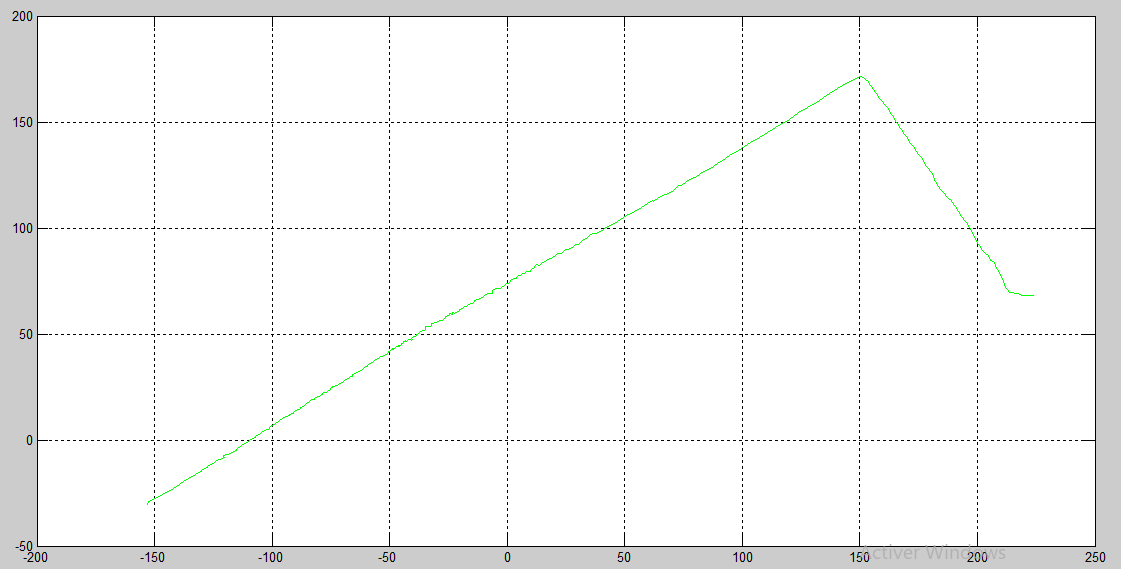
\includegraphics[scale=0.5]{graphedonnees.png}
	\captionof{figure}{\textit{Tracé des données du robot\\}}
	\label{fig2} 
	\end{center} 

\pagebreak
\section{\textsc{Identification par les moindres carrés basiques}}	

	\paragraph{}
	On sait que l'équation d'une droite est de la forme $ y=ax+b $ qu'on pourra illustrer aussi de cette manière :\\
	\begin{center}
		$ y = \begin{bmatrix} x&1 \end{bmatrix} \begin{bmatrix} a\\b \end{bmatrix} $ 
	\end{center}
	
	Arrivés là une identification avec la forme $ y = \varphi^{T}P $ est possible avec :
	  
	\begin{center}
		$ \varphi^{T} = \begin{bmatrix} x&1 \end{bmatrix} $ et $ P = \begin{bmatrix} a\\b \end{bmatrix}$
	\end{center}
	Ou $P$ correspond aux paramètres et $\varphi^{T}$ correspond au vecteur de régression. Le fichier ZT contient 			deux colonnes: colonne 1 pour les Y et colonne 2 	pour les X, donc on aura exactement N=507 mesures alors on 			parle de matrice de régression $\phi$ et pas que de vecteur de régression $\varphi$, avec $ \phi = 					\begin{bmatrix} \varphi^{T}_{1}\\.\\ \varphi^{T}_{i} \\.\\ \varphi^{T}_{N} \end{bmatrix} $ et $ Y = 					\begin{bmatrix} y_{1}\\.\\ y_{i} \\.\\ y_{N} \end{bmatrix} $ ,\label{section 1.2} \hyperref[Annexe A] {voir code 	Matlab en annexe}.
	
	\begin{center}
	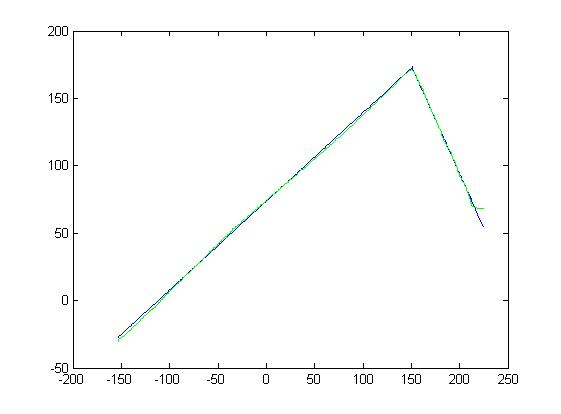
\includegraphics[scale=0.7]{2.jpg}
	\captionof{figure}{\textit{Tracé des droites modélisées par les MC basiques superposé avec celui des données\\}}
	\label{fig3} 
	\end{center}

	\textbf{Nota:} La détection de l'instant de commutation à i=417 nous a permis de tracer les deux modéles. \\[1cm] 
	
	\par Cette approche est limitée car elle traite un mur à la fois, autrement dit un modèle par mur. Mais comme la problématique abordée comporte plus d'un mur l'algorithme de cette approche risque d'être très long et quasiment impossible à coder pour une situation réelle ou on affronte une multitude d'obstacles (murs...etc). 
	

\section{\textsc{Identification par les moindres carrés récursifs}}
\subsection{\textsc{ Principe et ... }}

	\paragraph{} L'algorithme des moindres carrés récursifs se compose de deux parties, partie initialisation et partie calcul itératif des parmaètres. Il existe deux solutions pour initialiser cet algorithme, soit avec un choix arbitraire des paramètres ou bien de faire un petit prélévement des mesures donc celles du fichier ZT. Dans notre cas on se penchera plus tôt sur la deuxième option c'est à dire on prélève un nombre de mesures $N_0$ qui est égale dans notre cas à $3$ puis en utilisant les moindres carrés basiques on poura facilement trouver la matrice de régression $\phi_0$ ainsi que les paramètres $P_0$ et la matrice $A_0$ qui est égale à $\phi^{T}_{0} \phi_0$.\\
Le calcul itératif des paramètres consiste à acquérir à chaque itération une nouvelle mesure $y_{N+1}$, de calculer son $y_{MOD_{N+1}} = \varphi^{T}_{N+1} \hat{P}_N$
, \label{section 1.3.1} \hyperref[Annexe B] {voir code Matlab en annexe}. 